\documentclass[12pt]{article}
\usepackage[utf8]{inputenc}
\usepackage{indentfirst}
\usepackage{graphicx}
\renewcommand{\figurename}{Figura}
\usepackage{subcaption}
\usepackage{amsmath}
\graphicspath{ {fig/} }
\usepackage{geometry}
\geometry{top = 30mm}
\begin{document}
\section{Conversor DC-DC Buck}
\subsection{Análise teórica}
Este capitulo tem como objetivo analisar o conversor DC-DC Buck. Assim, será determinada a função transferência $\frac{V_{out}}{V_i}$ do conversor, que permitirá chegar a um fator de conversão, bem como a eficiência do mesmo. Esta analise será feita sem ter em conta as capacidades parasitas.
O conversor Buck está representado na figura  \ref{fig:Nucleo_do_conversor_DC-DC_Buck}.
\begin{figure}[htbp]
	\centering
	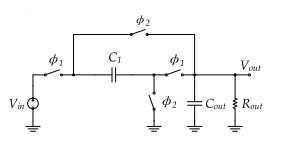
\includegraphics[height=2.5cm]{Buck}
	\caption{Núcleo do conversor DC-DC Buck}
	\label{fig:Nucleo_do_conversor_DC-DC_Buck}
\end{figure}

A análise do conversor será realizada em três instantes, em que cada um está associado a uma fase. Se o circuito estiver a funcionar na fase 1 ($\phi_1$) obtém-se o circuito representado na figura \ref{fig:Fase1}, mas se estiver a funcionar na fase 2 ($\phi_2$) obtém-se o circuito da figura \ref{fig:Fase2}.
	
\begin{figure}[htbp]
\centering
\begin{minipage}{.5\textwidth}
	\centering
	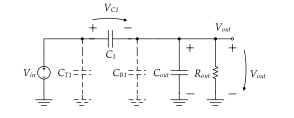
\includegraphics[width=1.1\linewidth, height=2.5cm]{Fase1}
	\caption{Fase 1 ($\phi_1$)}
	\label{fig:Fase1}
\end{minipage}%
\begin{minipage}{.5\textwidth}
	\centering
	\begin{equation}
		x+1=0
	\end{equation}					
\end{minipage}
\end{figure}

De forma a obter a relação $\frac{V_{out}}{V_i}$ considera-se que existe conservação de carga entre fases. Em ambos os casos existe conservação de carga no nó de saída e considerando o seguinte andamento temporal (figura \ref{fig:Andamento temporal}).

\begin{figure}[h]
	\centering
	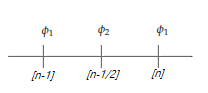
\includegraphics[height=2.5cm]{andamentotemporal}
	\caption{Andamento temporal}
	\label{fig:Andamento temporal}
\end{figure}
Considerando a conservação de carga da fase 1 para a fase 2 ($\phi_1 \rightarrow \phi_2$) obtém-se a seguinte equação.
\vspace{5mm}

\begin{equation}
\label{eq:Fase1to2}
Q^{\phi_2}_{C_1} + Q^{\phi_2}_{C_{out}} + \Delta Q_{Rout} = Q^{\phi_1}_{C_1} + Q^{\phi_1}_{C_{out}} 
\end{equation}
\vspace{5mm}

Tendo em consideração que $\Delta Q_{Rout} = \frac{T_{clk} }{2}I_{out}$ a equação \ref{eq:Fase1to2} pode ser escrita da seguinte forma:

\begin{equation}
\label{eq:Fase1to2s}
V_{out}[n-\frac{1}{2}]C_1 + V_{out}[n-\frac{1}{2}]C_{out} +  V_{out}[n-\frac{1}{2}](\frac{T_{clk} }{2}\frac{1}{R_{out}})=(V_i-V_{out}[n-1])C_1 + V_{out}[n-1]C_{out}
\end{equation}
\vspace{5mm}

Considerando agora a conservação de carga da fase 2 para a fase 1 ($\phi_2 \rightarrow \phi_1$) obtém-se a seguinte equação.

\begin{equation}
-Q^{\phi_1}_{C_1} + Q^{\phi_1}_{C_{out}} + \Delta Q_{Rout} = -Q^{\phi_2}_{C_1} + Q^{\phi_2}_{C_{out}}
\end{equation}

\begin{equation}
\label{eq:Fase2to1}
-(V_i-V_{out}[n])C_1+ V_{out}[n]C{out}+ V_{out}[n](\frac{T_{clk} }{2}\frac{1}{R_{out}}) = - V_{out}[n-\frac{1}{2}]C_1 + V_{out}[n-\frac{1}{2}]C_{out} 
\end{equation}
\vspace{5mm} 

Resolvendo a equação \ref{eq:Fase2to1} em ordem a $V_{out}[n-\frac{1}{2}]$ e substituindo na equação \ref{eq:Fase1to2s} obtém-se a seguinte expressão de $\frac{V_{out}}{V_i}$.
\begin{equation}
\label{eq:Buck(vo/vi)}
\frac{V_{out}}{V_i} = \frac{C_1(2 + \frac{T_{clk}}{2}\frac{1}{C{out}R_{out}})}{4C_1+ \frac{C_1T{clk}}{C{out}R_{out}} +  \frac{T_{clk}}{R_{out}} + \frac{T{clk}^2}{4R_{out}^2C_{out}} }
\end{equation}
\vspace{5mm} 

Considerando $C_{out}>> C_1$ e que $F_{clk} = \frac{1}{T{clk}}$ obtém-se:
\vspace{5mm}     

\begin{equation}
\label{eq:Buck(vo/vi)ap}
\frac{V_{out}}{V_i} = \frac{2F_{clk}R_{out}C_1}{4F_{clk}R_{out}C_1+ 1}
\end{equation}
\vspace{5mm}  

Como $4F_{clk}R_{out}C_1 > 1$ então: 

\begin{equation}
\label{eq:Buck(vo/vi)f}
\frac{V_{out}}{V_i} = \frac{1}{2}
\end{equation}
\vspace{5mm}  
Assim sendo, a razão de conversão do conversor é de $\frac{1}{2}$.

Através da equação \ref{eq:Buck(vo/vi)ap} é possível chegar á $F_{clk}$ do conversor.
\begin{equation}
\label{eq:FBuck(vo/vi)}
F_{clk}=\frac{V_{out}}{2R_{out}C_{1}(V_i-2V_{out})}
\end{equation}
\vspace{5mm}
A eficiência do conversor é dada por: $\eta = \frac{P_{out}}{P_{i}}$ onde $P_{out} = V_{out}I_{out}$ e $P_{in} = V_{i}I_{i}$
%\begin{equation}
%\label{eq:EfBuck(vo/vi)}

\begin{center}
{\large $\eta = \frac{P_{out}}{P_{in}} = \frac{ V_{out}I_{out}}{ V_iI_i} = \frac{|V_{out}(\Delta Q^{\phi_1}_{out} + \Delta Q^{\phi_2}_{out})F_{clk}|}{{|V_i(\Delta Q^{\phi_1}_{i} + \Delta Q^{\phi_2}_{i})F_{clk}|}}$}
\end{center}

%\end{equation}

\[\left\{
  \begin{array}{lr}
    x^2 & : x < 0\\
    x^3 & : x \ge 0
  \end{array}
\right.
\]

\begin{equation}
  \begin{array}{rrr}
    a + b + c & = & d \\        e + f     & = & g \\        h         & = & i
  \end{array}
\end{equation}

\begin{equation}
  \begin{aligned}
    a + b + c & =  d \\        e + f     & =  g \\        h         & =  i
  \end{aligned}
\end{equation}


\end{document} 